\chapter{Szerveroldali folyamatok implementációi}

A megjelenítési réteg alatt található szerveroldali folyamatok implementációja során a kiszolgáló infrastruktúra kialakítására, a Node.js-alkalmazás fejlesztésére, a konténerizált környezet kialakítására, valamint a videófeldolgozásra fókuszálunk ebben a fejezetben.

\section{A virtuális privát felhő komponensei}

A szerveroldal erőforrásait igyekeztem mindet egy közös VPC-be szervezni, amely lehetővé teszi, hogy a komponensek egymást lássák, és biztonságosan kommunikáljanak egymással alhálózataik között. A VPC-n belül az összetartozó elemekhez két-két alhálózatot hoztam létre. A legtöbb AWS-szolgáltatás a magas rendelkezésreállás érdekében legalább kettő konkrét adatközpontba kell kitelepítése kerüljön, azaz az AWS saját terminológiáját használva: két \emph{Availibility Zone}-ba (AZ) kell elhelyezésre kerüljenek a konkrét erőforrások. Ennek megfelelően az eu-central-1 régió alatti \emph{eu-central-1a} és \emph{eu-central-1b} AZ-ba szerveztem az egyes alhálózataim. Az alhálózatok közötti forgalom irányítását útválasztó táblák (angolul \emph{route table}) segítségével végeztem, amelyek biztosítják, hogy a komponensek közötti kommunikáció megfelelően működjön. Az útválasztó táblák konkrét bejegyzéseit, valamint a felhasznált IP-tartományokat is tartalmazza a \refstruc{fig:vpc}.

\begin{figure}[ht]
  \centering
  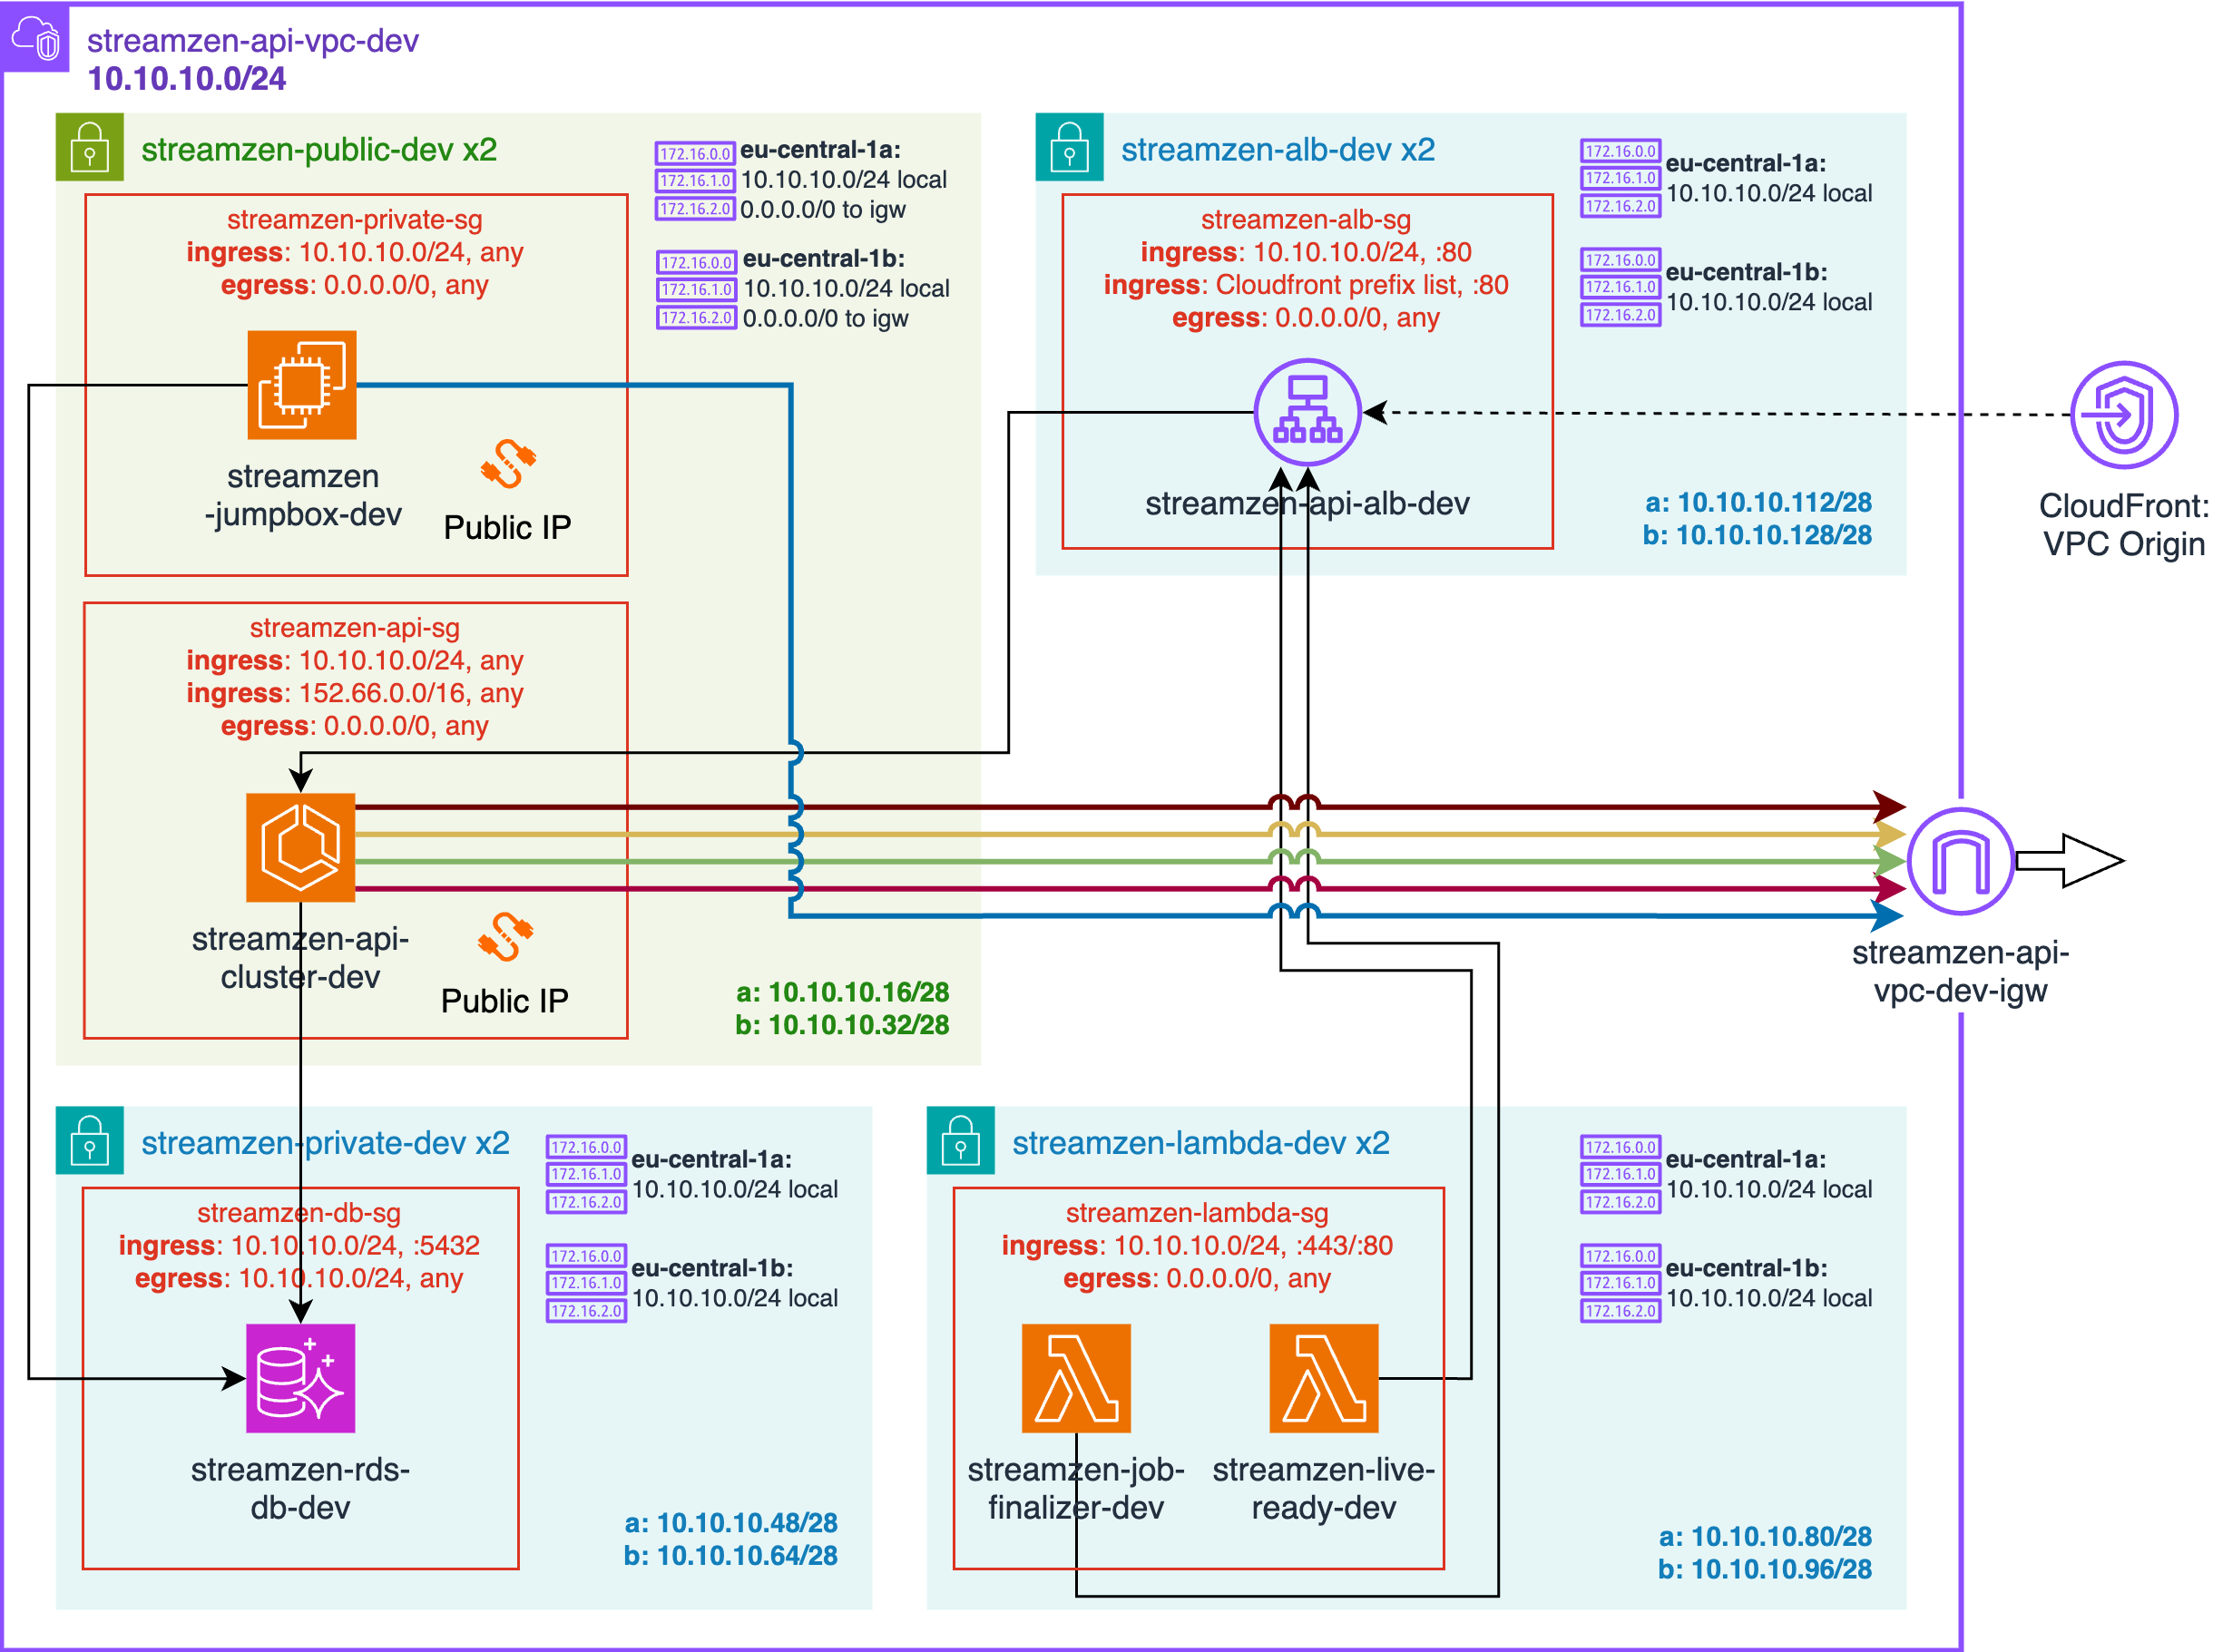
\includegraphics[width=150mm, keepaspectratio]{figures/dipterv_vpc.png}
  \caption{Részletes architektúraábra a VPC-ről.}
  \label{fig:vpc}
\end{figure}

Az ábráról leolvashatóak még a Security Groupok, azaz virtuális állapotmentes tűzfalak, ezek a komponensek vörös keretként látszódnak az ábrán és \emph{-sg} végződésűek neveik. Ezek a tűzfalak úgy kerültek kialakításra, hogy a csupán a ténylegesen szükséges IP-tartományokat és portokat engedélyezzék a kommunikációhoz.

A legelső belépési pontja egy kérésnek az ALB-példány, amely privát alhálózatra lett bekötve. Privátnak minősül egy alhálózat, amennyiben nincs közvetlen internetkapcsolata, nem kerül bekötésre az útválasztó táblájába IGW.

Habár bevezetésre került egy Internet Gateway (IGW), fontos megjegyezni, hogy nem azért, hogy a kliensoldali erőforrás -- a CloudFront-disztribúció -- elérhesse a szerveroldalt, hiszen azt megvalósítja egy VPC Originen keresztül, amely működési lényege, hogy számára nem szükségeltetik bevezetni publikus alhálózatot, a disztribúció közvetlen összeköttetést tud összehozni VPC-n belül elrejtett hálózati erőforrásokkal, azaz a mi ALB-példányunkkal is. Az IGW bevezetésének indokait a következő bekezdések tisztázzák.

Az ECS-klaszter, amely a Node.js-alkalmazást futtatja és összeköttetésre kerül az ALB-vel, viszont már publikus alhálózatban helyezkedik el. A Security Groupja úgy lett beállítva, hogy a VPC-n belüli eszközöket engedje be, illetve azt az IP-tartományt, amelyben az AuthSCH is fut (ez a Schönherz Kollégium hálózati tartománya, a 152.66.0.0/16).

A szervernek fontos a kapcsolódása az adatbázisra, amely egy külön privát alhálózatot kapott, abba a Security Group csupán a PostgreSQL-re jellemző 5432 porton keresztül enged és csak a VPC-belülről forgalmat, hasonlóképp kifelé is csak a VPC-n belülre enged.

Az ECS-klaszterben működő szervernek több külhálózaton működő szolgáltatás felé kell tudnia kommunikálni. Ezek a VPC-n kívüli komponensek a \refstruc{fig:nonvpc} segítségével kerülnek vizuálisan ismertetésre.

\begin{figure}[ht]
  \centering
  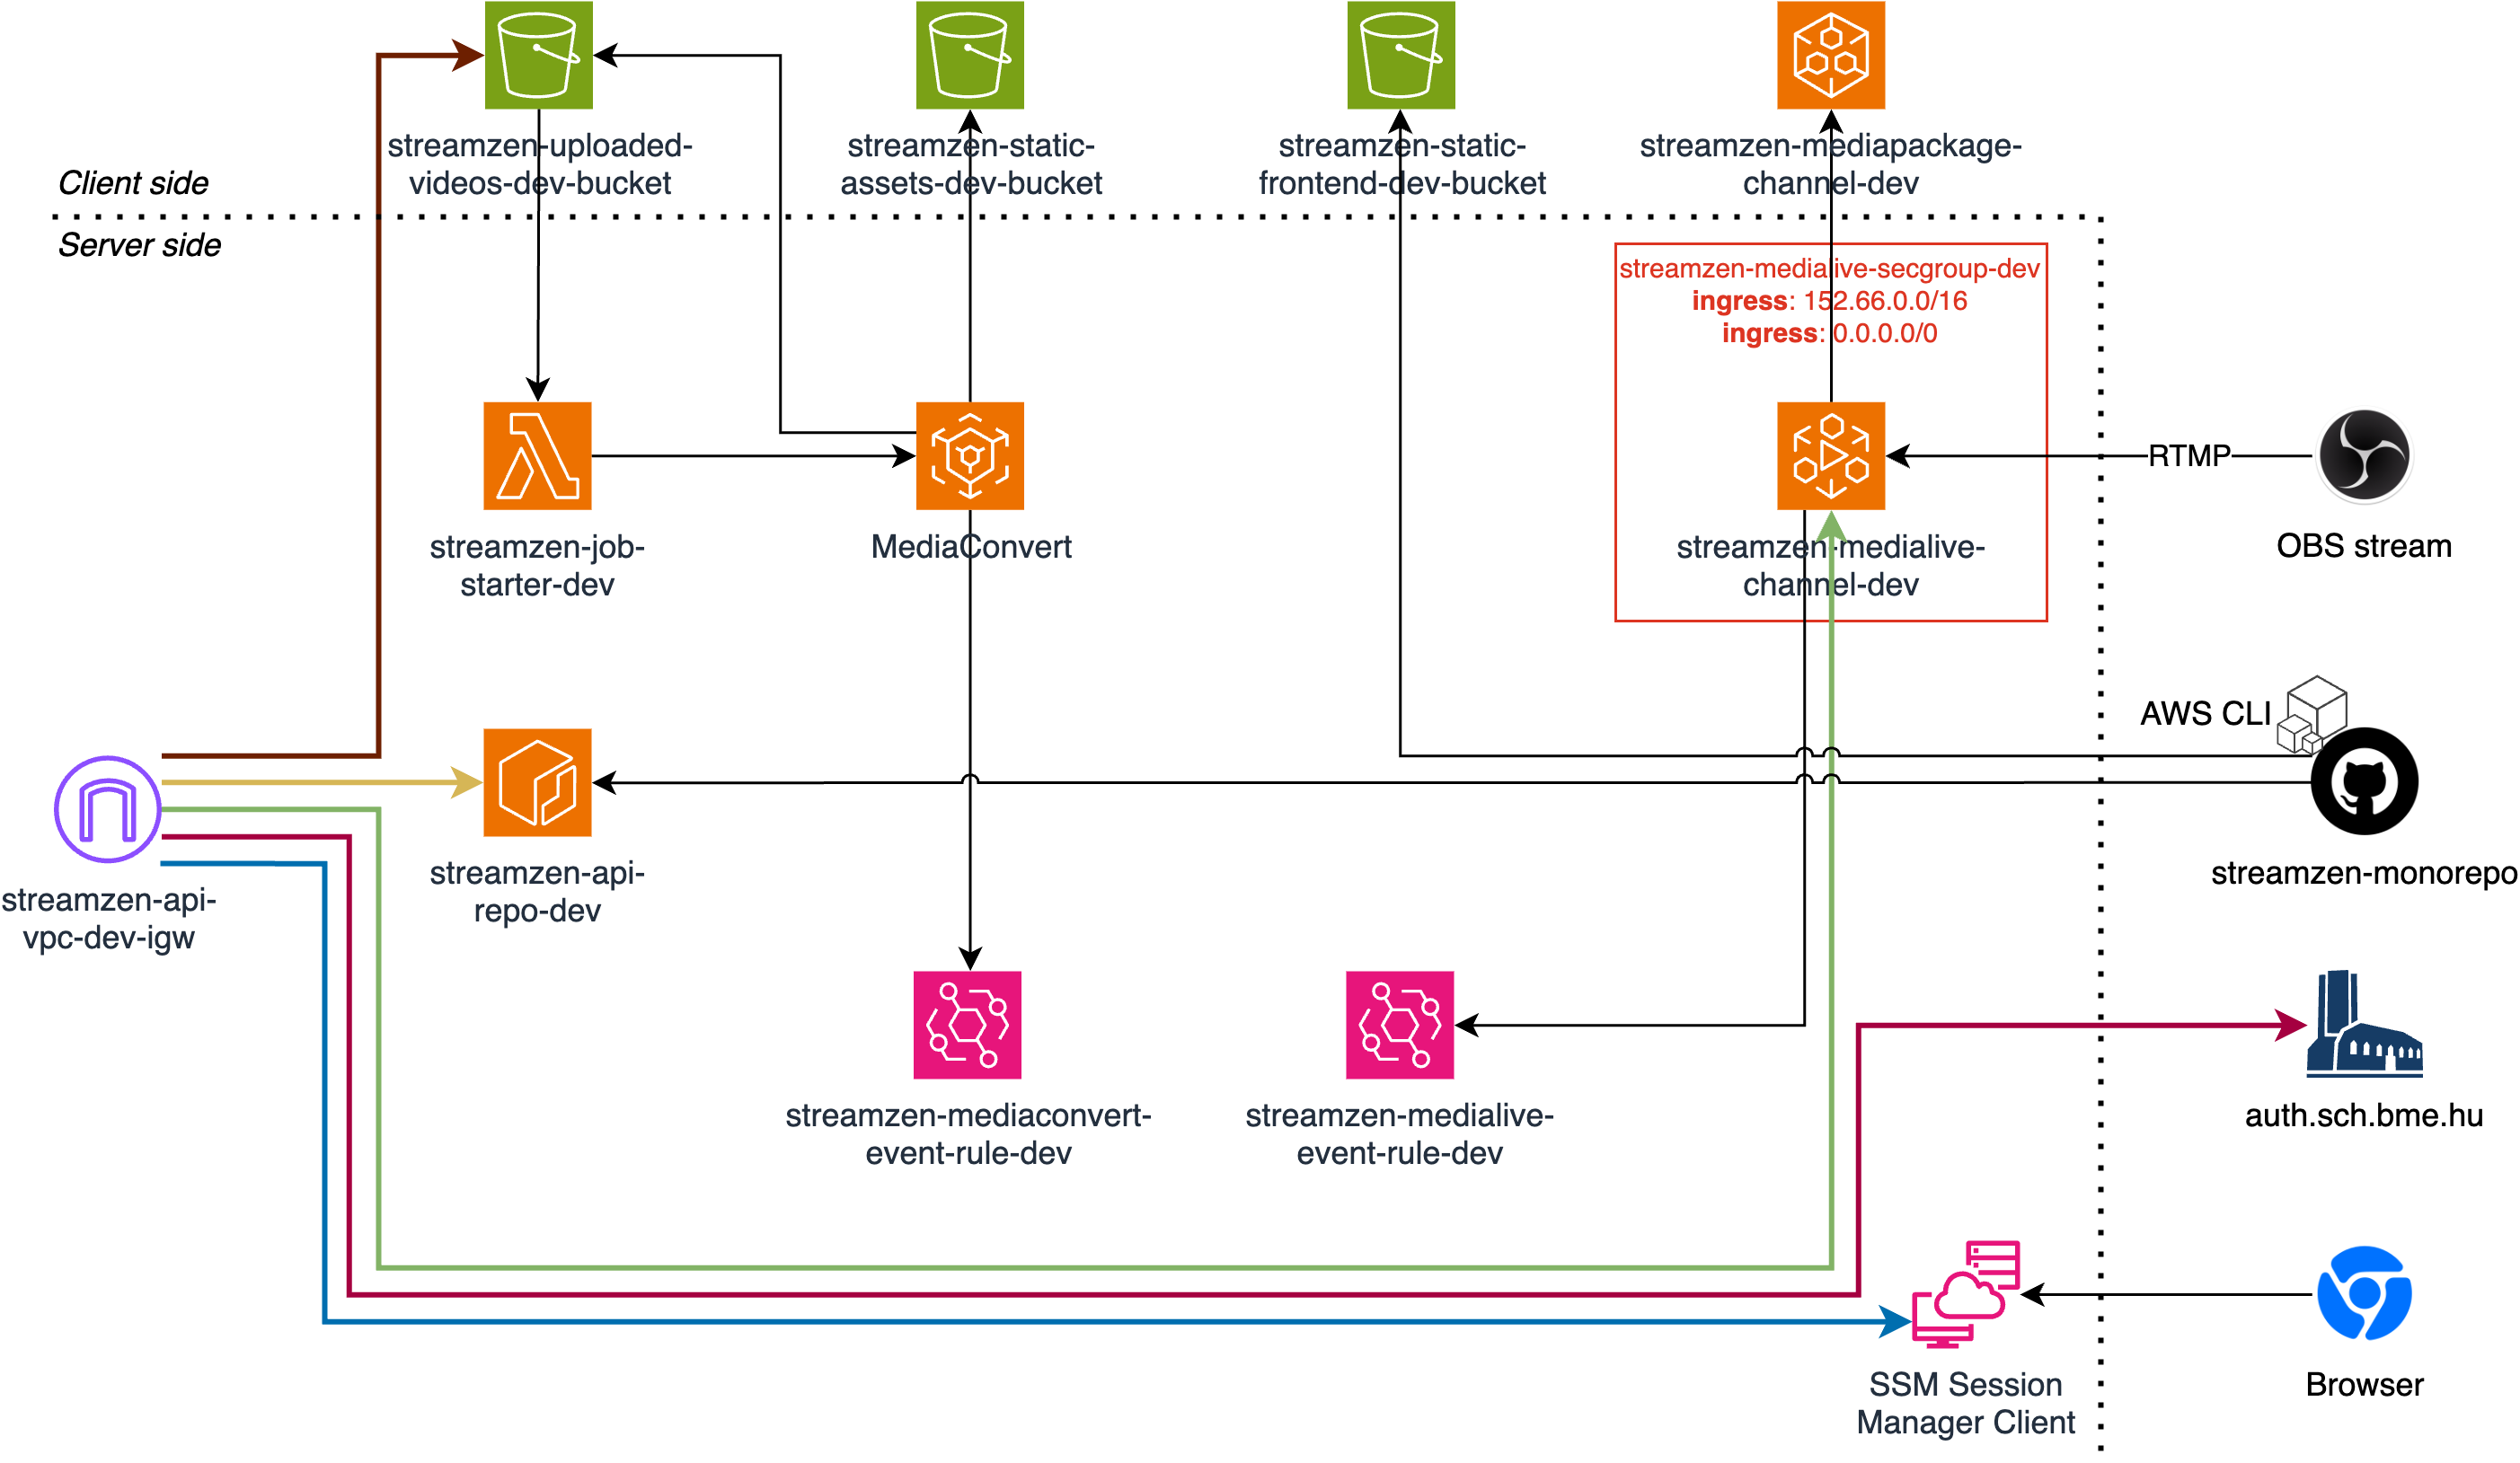
\includegraphics[width=150mm, keepaspectratio]{figures/dipterv_nonvpc.png}
  \caption{Részletes architektúraábra a VPC-ből kifelé és befelé kommunikáló komponensekkel.}
  \label{fig:nonvpc}
\end{figure}

A \refstruc{fig:nonvpc} ábra és a \refstruc{fig:vpc} együttesen mutatja be az Internet Gateway-en keresztüli kommunikációs útvonalakat, azonos színű vonalak egyazon kommunikációs útvonalat jelölik. Ennek megfelelően az előző bekezdésben jelölt AuthSCH-t elérő kommunikációs útvonalat jelöli a piros vonal. A sárga vonal jelöli azt, ahogy az ECS-klaszter eléri az ECR-repository-t a Docker-kép letöltésére. A zöld vonal jelöli a szerver és a MediaLive-csatorna közti utat, amelyen keresztül a szerver elindítja az vételt a csatornán. Végül pedig a barna vonal jelöli a videófeltöltés folyamatát az S3-vödörbe a szerveren keresztül.

Léteznek különféle hálózati erőforrástípusok, hogy privát alhálózatban helyezzünk el egy ECS-ben futó szervert, illetve akár Lambda-függvényeket, amelyek kommunikálnak VPC-n kívüli eszközökkel. Ilyen erőforrástípus a \emph{NAT Gateway}, amely Network Address Translation (NAT) szolgáltatás, és amennyiben adunk neki egy állandó publikus IP-címet (Amazon Elastic IP szolgáltatással), úgy képes azon keresztül az internet felé forgalmazást biztosítani a VPC erőforrásai számára, kinti erőforrásoknak viszont befelé már nem. Ez megoldotta volna az AuthSCH felé kommunikálást. Egy másik lehetőség lett volna a \emph{VPC Endpointok} alkalmazása, amelyek interfészt szolgáltatnak bizonyos AWS-en belüli szolgáltatások felé anélkül, hogy az elhagyná az adatközpontot. A bizonyos szolgáltatások közé tartozik a CloudWatch Logs, az ECR, az ECS-hez tartozó egyéb szolgáltatások, az EventBridge és az S3 is. Ezt a biztonsági kockázatot a kísérletem szempontjából nem kívántam megelőzni, az igazán szükséges védelmi réteget a Security Group is megvalósítja, a privát alhálózat csupán plusz egy réteget jelent nagy kockázatú, vegyes forgalmat kezelő enterprise rendszerek kivitelezése során, az én esetemben a költségek és a bonyolultság erősen megnőtt volna jelölt erőforrások bekötésével.

A hálózat építése tégláról téglára került kivitelezésre, a fejlesztési/tervezési fázisban ezért érdemesnek tartottam a tesztelés során \emph{``jumpbox''} jelleggel bevezetni egy EC2-példányt, amely a publikus alhálózatban helyezkedik el. Viszont az elérése nem kívántam jelszavakat, SSH-kulcsokat kezelni, ezért az AWS Systems Manager (SSM) Session Manager szolgáltatását használtam, amely lehetővé tette, hogy a webes konzolon keresztül SSH-kapcsolatot létesítsek az EC2-példánnyal anélkül, hogy közvetlenül elérné azt. Az EC2-es példány létrehozása után egy ágenset kellett volna telepítsek, amely erre felkészíti magát a virtuális gépet, azonbna ezt a telepítési folyamatot is automatizáltam a Systems Manager Host Management szolgáltatásával, a \ref{fig:hostmgmt} ábra mutatja be a Host Management gyorstelepítési oldalát, amely lehetővé teszi az EC2-példányok központi kezelését. A jumpbox segítségével tudtam pingelgetni a hálózati eszközök interfészeit, illetve a Security Groupok beállításait is tesztelni, és akár az RDS-adatbázison is futtatni egyszerű lekéréseket, sémamigrációkat.

\begin{figure}[ht]
  \centering
  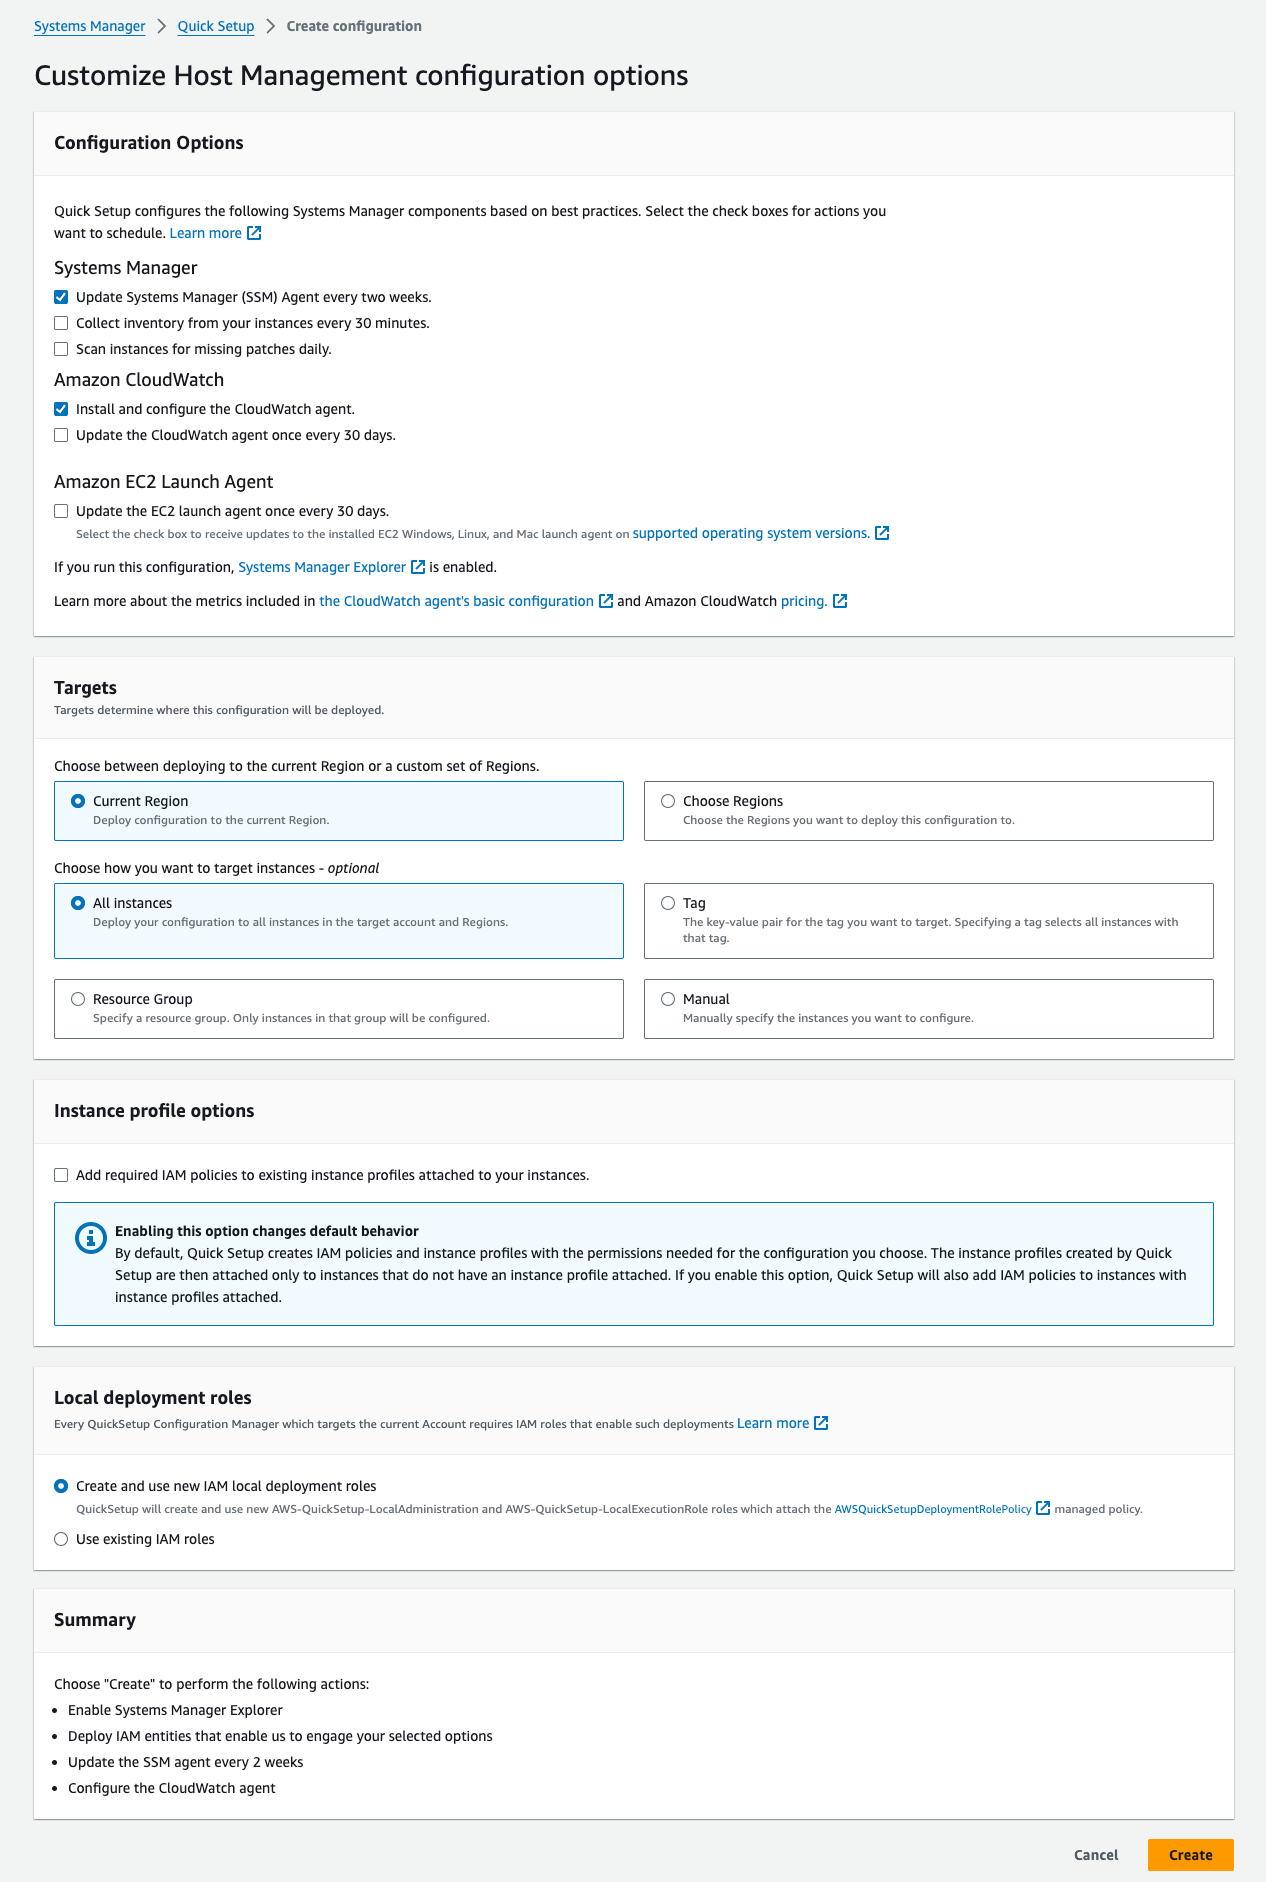
\includegraphics[width=152mm, keepaspectratio]{figures/hostmgmt.png}
  \caption{A Host Management gyorstelepítési oldala.}
  \label{fig:hostmgmt}
\end{figure}

\section{A Node.js-alkalmazás fejlesztése}

TODO: Az elkészült alkalmazás felépítése, a különböző rétegek, a routing, a middleware-ek, a kontrollerek, a service-ek, a REST API.

\subsection{Az adatbázisséma}

A \refstruc{fig:prismaliser} mutatja be a Prisma-ban írt Prisma-sémát. A séma tartalmaz jövőbeli felhasználásra szánt elemeket, az egyszerűségre törekszik a séma, csupán a lényeges adatokat tároljuk le.

\begin{figure}[!ht]
  \centering
  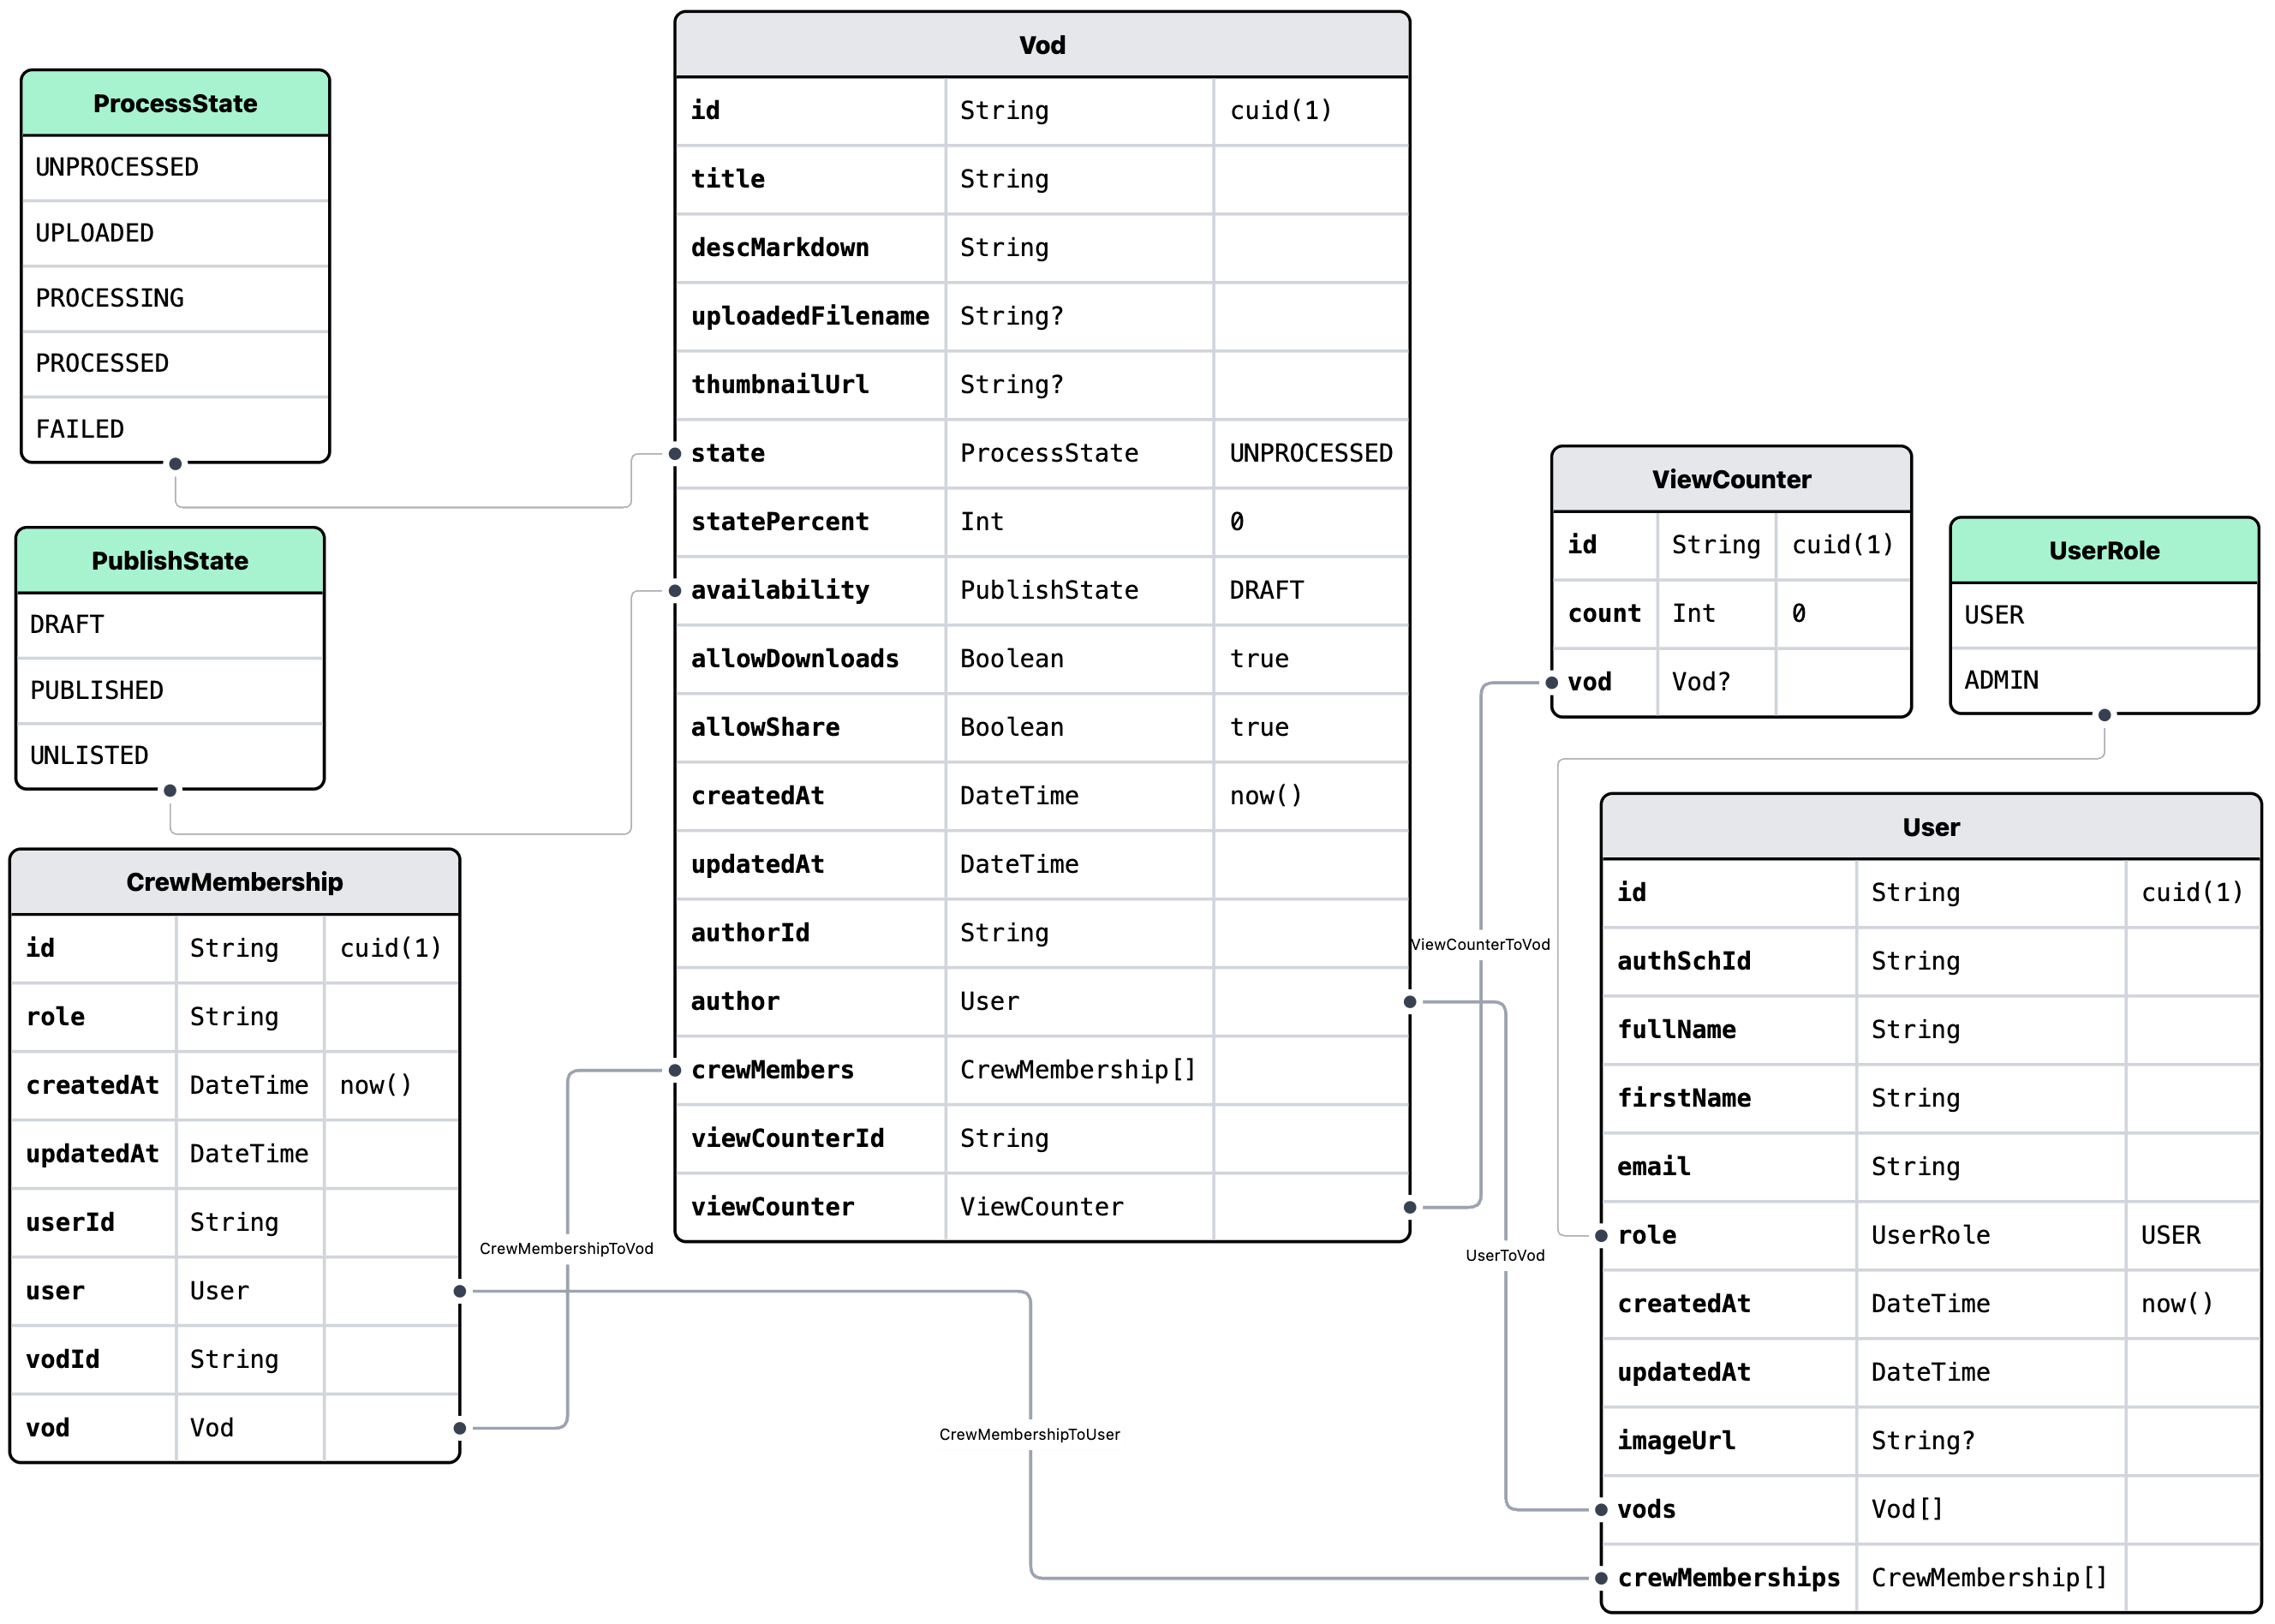
\includegraphics[width=155mm, keepaspectratio]{figures/prismaliser.png}
  \caption{A Prisma-séma vizuális reprezentációja.}
  \label{fig:prismaliser}
\end{figure}

A User entitás reprezentálja a felhasználókat, akik megfelelő role attribútumérték esetén feltölteni tudnak a weboldalra. A role attribútum típusát enum típusra állítottam, amelynek értékei a \verb|USER| és \verb|ADMIN|. A Usernek számított attribútuma a vods és a crewMemberships.

A Vod entitás a feltöltött videók metaadataid reprezentálja. A Vod entitásnak meg kell adni létrehozáskor egy User kapcsolatot, amely a feltöltő felhasználót reprezentálja. Ezenkívül fontos attribútuma a state, amely a videó állapotát reprezentálja. A state attribútum enum típusú, lehet értéke \verb|UNPROCESSED| (ez a létrehozáskori érték), lehet \verb|UPLOADED| (amikor feltöltésre került), \verb|PROCESSING| (amikor már a MediaConvert dolgozik az átalakításán), \verb|PROCESSED| (amikor véget ért a MediaConvert-job), vagy pedig \verb|FAILED| (amennyiben hiba történt valamelyik fázisban). Segít a videó állapotának nyomon követésében a statePercent attribútum is, amely a MediaConvert által visszaadott százalékos értéket tárolja le.

A CrewMembership entitáshoz tartozó tábla a Vod és a User entitások közötti illesztő tábla (angolul \emph{join table}), saját attribútumokat tud ehhez a kapcsolathoz hozzáadni, kardinalitás szempontjából egy CrewMembershipnek csak egy Usert és csak egy Vodot kell kötnie. Egy Vodnak persze több CrewMembershipje is lehet, ugyanígy Usernek is. Ez az entitás és a ViewCounter -- amely a megtekintések számlálóját lett volna hivatott reprezentálni -- aktívan nem került felhasználásra a fejlesztés során, tervezésben maradt csupán, nem volt esszenciális a végső cél megvalósításához.

\subsection{Környezeti változók}

Az alkalmazásnak korábbi alfejezetekben már kiderült, hogy vannak külső függőségei. Ezen függőségekhez való hozzáféréshez a környezeti változók használata elengedhetetlen. A ECS-ben futó konténer környezeti változóinak beállítására az ECS is ad lehetőséget a \ref{lst:mainApi}. kódrészlet mutatja be a Terraform-kód egy részletét, amely átpasszolja az alkalmazás számára a következő fontos paramétereket.

Az AuthSCH SSO-ban felvett kliensünk azonosítóját és titkos kulcsát a \verb|AUTHSCH_CLIENT_ID| és \verb|AUTHSCH_CLIENT_SECRET| környezeti változók tárolják, ezek értékeit ahogy a kódból is látható egy-egy SSM Parameter Store-ból szerzi meg a CI/CD-folyamat futtatása során a Terraform-kliensünk (értsd: a referált erőforrás elején \verb|data| kulcsszó jelöli, hogy \emph{data source}-ként éri kéri le a Terraform az AWS CDK-n keresztül az értékét). Ezen Param Store kulcs-érték párokhoz az értéket az AuthSCH saját oldalán szereztem meg \url{https://auth.sch.bme.hu} oldalon található webes felületén, ahol korábban már megszerzett SCHacc-fiókomba való belépés után új OAuth-kliens beregisztrálása után tudtam magamnak generálni a kívánt értékeket (ID és client secret).

A PostgreSQL-adatbázis felhasználónevét és jelszavát (\verb|POSTGRES_USER| és \verb|POSTGRES_PASSWORD|) is meg kell tudjuk adni környezeti változón keresztül az alkalmazásunknak, ezek értékét is SSM Param Store-okba tettem bele, viszont a felhasználónevet már magam találtam ki, a jelszót pedig magam generáltam kézzel.

Az alkalmazásnak tudnia kell bizonyos átirányítások lekezelésére a kliensünk bázis URL-jét, így azt megadtam környezeti változóban (\verb|FRONTEND_CALLBACK|). A doménnevet változtathatónak véltem hagyni, ezért is került Terraform-változóba az értéke (\verb|var.domain_name|).

Ezenkívül még szükség van egy titkos kulcsra, amely a JWT-tokenek aláírására szolgál (\verb|JWT_SECRET|), ezt is SSM Param Store-ból szerzi be az alkalmazásunk, illetve ezt is már én töltöttem be, miután kézzel generáltam egyet.

A feltöltött videókat tároló S3-vödör nevét (\verb|AWS_S3_UPLOADED_BUCKET|) az általam kitalált nevezéktani konvenciók alapján töltöm be, illetve az S3-vödör régióját (\verb|AWS_S3_REGION|) pedig természetesen arra a régióra állítom, ahová az erőforrások főképp telepítésre kerültek (és ahova az S3-vödör is került). 

\begin{minipage}{0.92\textwidth}
  \begin{lstlisting}[
    caption=Az ECS-szerveralkalmazás környezeti változóinak feltöltése a main.tf fájlban.,
    label=lst:mainApi,
    style=tf,
    basicstyle=\fontsize{10}{12}\ttfamily,
  ]
task_environment = {
  AUTHSCH_CLIENT_ID = data.aws_ssm_parameter.these["authsch-client-id"].value
  AUTHSCH_CLIENT_SECRET = data.aws_ssm_parameter.these["authsch-client-secret"].value
  POSTGRES_USER = data.aws_ssm_parameter.these["db-username"].value
  POSTGRES_PASSWORD = data.aws_ssm_parameter.these["db-password"].value
  FRONTEND_CALLBACK = "https://${var.domain_name}"
  JWT_SECRET = data.aws_ssm_parameter.these["api-jwt-secret"].value
  AWS_S3_REGION = var.region
  AWS_S3_UPLOADED_BUCKET = "streamzen-uploaded-videos-${var.environment}-bucket"
}
\end{lstlisting}
\end{minipage}

\subsection{A videófeltöltés üzleti logikája}

A szerveroldalon kialakításra kerülő konkrét üzleti logikai folyamatok közül a feltöltésre kerülő nyers videók S3-vödörbe való továbbítása az egyik legérdekesebb. A fentebb ismertetett VideoController és VideoService osztályokból emeli ki rendre a \ref{lst:videoController}. kódrészlet és a \ref{lst:videoService} kódrészlet a fontosabb részeket.

\begin{minipage}{0.92\textwidth}
  \begin{lstlisting}[
    caption=Videófeltöltés kezelése a VideoController osztályban.,
    label=lst:videoController,
    style=js,
    basicstyle=\fontsize{10}{12}\ttfamily
  ]
@Post(":id/upload")
@UseGuards(JwtGuard)
@UseInterceptors(FileInterceptor("file"))
async upload(
  @Param("id") id: string,
  @UploadedFile(new ParseFilePipe()) file: Express.Multer.File
) {
  const { originalname, buffer } = file
  const res = await this.videoService.upload(id, originalname, buffer)
  return await this.videoService.afterUpload(id, res.fileName)
}
\end{lstlisting}
\end{minipage}

A feltöltéshez szükséges fájlok a kliensoldalon kerülnek kiválasztásra, és a POST metódusú \verb|/api/videos/:id/upload| végponton keresztül kerülnek feltöltésre. Ezt a végpontot hallgatja le a \verb|VideoController| osztálybéli \verb|upload| függvény is. A függvény dekorátorai közül a \verb|@Post| jelöli azt, amiképp hallgat a kérésekre (POST metódussal és a jelölt útvonalon). A \verb|@UseGuards| dekorátor az autentikáció szükségességét biztosítja a kérések végbemeneteléhez, amelyet a mi esetünkben a \verb|JwtGuard| osztály valósít meg. A \verb|@UseInterceptors| dekorátor pedig egy interceptort állít be a függvény elé, a fájlok feltöltését segíti elő, amelyet a \verb|FileInterceptor| osztály valósít meg. Ez az osztály a NestJS alatt működő Express keretrendszerben működő \emph{Multer} nevű Node.js-middleware-t hasznosítja, amellyel így tehát képes az osztály mögötti logika a HTTP-alapú bájtfolyamot hatékonyan feldolgozni/parse-olni, és elrejteni előlünk a sok-sok kihívását egy fájlfeltöltésnek. A függvény paramétereiben a \verb|file| paraméter a \verb|@UploadedFile| dekorátoron keresztül válik a feltöltött fájl reprezentációjává, típusa is a \verb|File| interfész lesz.

A VideoService-ben működő \verb|upload| függvény felé lesz a kapott fájl bufferje továbbítva, végül a service-függvény eredményéből született fájlnévvel kerül az adatbázisba is lementésre az entitásként a videó is a \verb|afterUpload| függvény által.

\begin{minipage}{0.92\textwidth}
  \begin{lstlisting}[
    caption=Videófeltöltés függvénye a VideoService osztályban.,
    label=lst:videoService,
    style=js,
    basicstyle=\fontsize{10}{12}\ttfamily
  ]
private readonly s3Client = new S3Client({
  region: this.configService.getOrThrow("AWS_S3_REGION"),
})
async upload(id: string, fileName: string, file: Buffer) {
  const ext = fileName.split(".").slice(-1)[0]
  const baseName = new Date()
    .toISOString().slice(0, 19).replaceAll(":", "-")

  const response = await this.s3Client.send(
    new PutObjectCommand({
      Bucket: this.configService.getOrThrow("AWS_S3_UPLOADED_BUCKET"),
      Key: `${id}/${baseName}.${ext}`,
      Body: file,
    })
  )
  return { ...response, fileName: `${baseName}.${ext}` }
}
\end{lstlisting}
\end{minipage}

A VideoService az AWS SDK S3 API-ját használja a fájlok vödörbe való feltöltésére. Ehhez létrehoztam tagváltozóként a \verb|s3Client|-et. A \verb|upload| függvény először átalakítja a fájlnevet, megtartja a kiterjesztést, viszont a dátumot szerkeszti bele a konkrét névbe. Majdpedig készít egy \verb|PutObjectCommand| típusú objektumot, amellyel a megfelelő helyre és névvel kerül feltöltésre az \verb|s3Client|-en keresztül a fájl.

\section{A konténerizált környezet}

TODO: Leírás, hogy miért választottam a konténerizált környezetet, a konténerizálás előnyeit, hátrányait. Hogy használható ki a legjobban a konténerizáció az Application Load Balancer-rel együtt. Miképp kapcsoltam ezt a kettőt össze (ECS service, ALB).

TODO: Az ECS orkesztrációs toolsetjének kialakítása, a konténer rétegződés felépítése ECS-ben, a konténer registry (ECR) bekötése. Környezeti változók, portok, ALB-re való kötése. Miből állt a dockerizálás nekem (Dockerfile, registry, image build, push, networking).

\begin{figure}[ht]
  \centering
  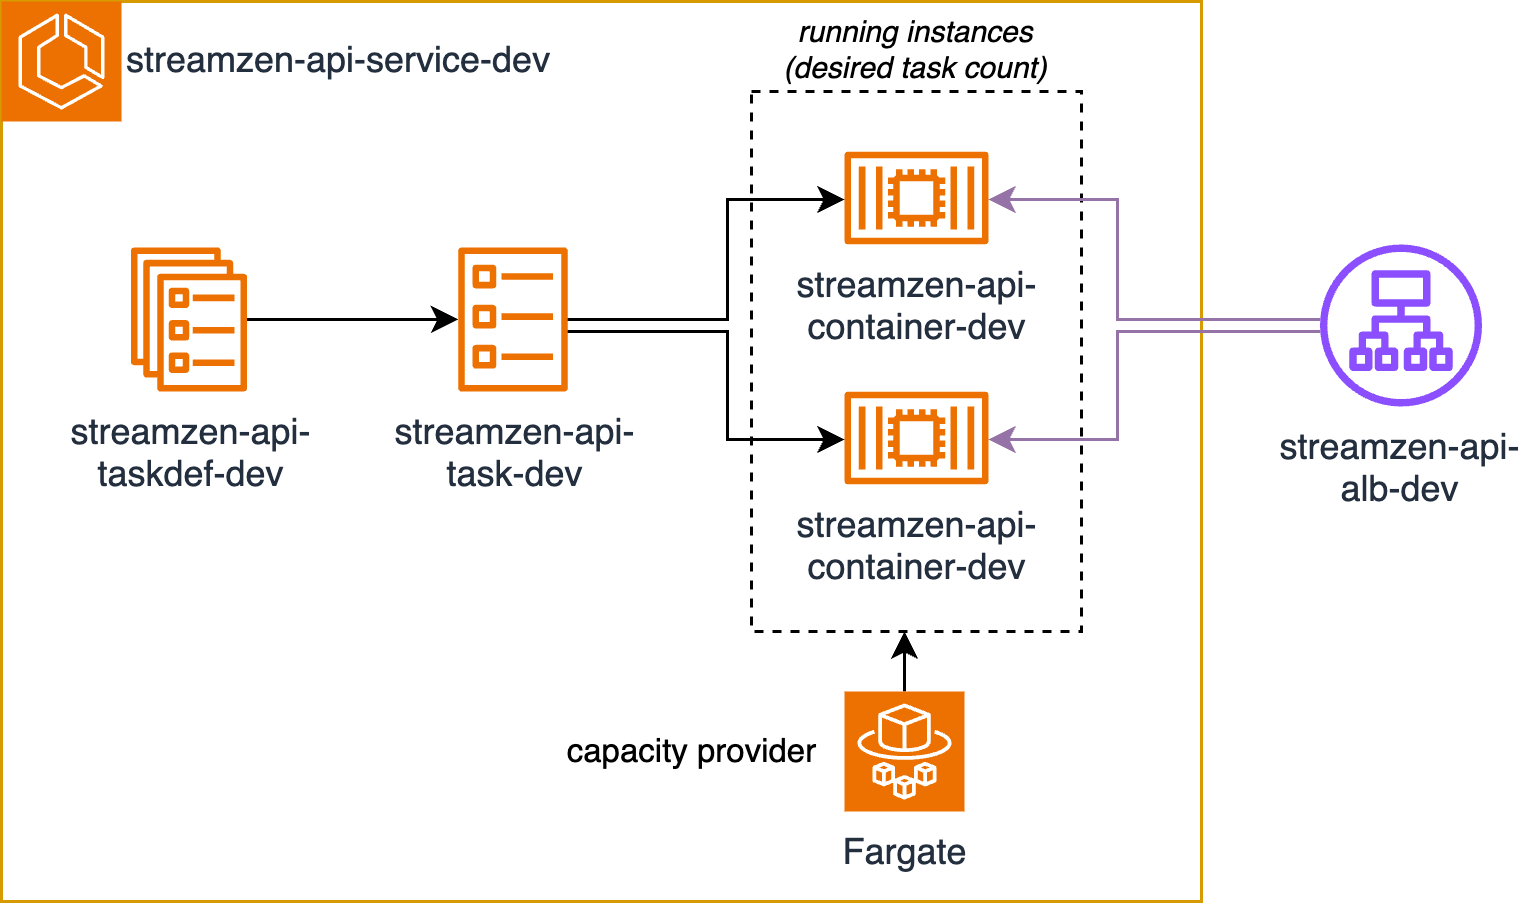
\includegraphics[width=150mm, keepaspectratio]{figures/dipterv_ecs.png}
  \caption{Az ECS-klaszter elemei.}
  \label{fig:ecscluster}
\end{figure}

\begin{minipage}{0.92\textwidth}
  \begin{lstlisting}[
    caption=Az ECS-klaszter és -szolgáltatás konfigurációja az api-stack modul alatti ecs.tf fájlban.,
    label=lst:ecsCluster,
    style=tf,
    basicstyle=\fontsize{10}{12}\ttfamily
  ]
resource "aws_ecs_cluster" "this" {
  name = "streamzen-api-cluster-${var.environment}"
}
resource "aws_ecs_service" "this" {
  name            = "streamzen-api-service-${var.environment}"
  cluster         = aws_ecs_cluster.this.arn
  task_definition = aws_ecs_task_definition.this.arn
  desired_count   = var.ecs.desired_task_count
  launch_type     = "FARGATE"

  health_check_grace_period_seconds = 300
  network_configuration {
    subnets          = var.api_subnet_ids
    security_groups  = var.api_secgroup_ids
    assign_public_ip = true # false if you have a NAT GW
  }
  load_balancer {
    target_group_arn = aws_lb_target_group.this.arn
    container_name   = "streamzen-api-${var.environment}"
    container_port   = var.ecs.port_mapping
  }
}
\end{lstlisting}
\end{minipage}

TODO: kicsi magyarázat arról, hogy mire jó a processing power állítgatása. Itt lehet már beállítani, hogy honnan jön az image, és beállítod az ECR-t.

\begin{minipage}{0.92\textwidth}
  \begin{lstlisting}[
    caption=Az ECS-taszk definíciója az api-stack modul alatti ecs.tf fájlban.,
    label=lst:ecsTask,
    style=tf,
    basicstyle=\fontsize{10}{12}\ttfamily
  ]
resource "aws_ecs_task_definition" "this" {
  family                = var.ecs.family_name
  container_definitions = jsonencode([{
    volumes          = []
    mountPoints      = []
    healthCheck      = try(var.ecs.health_check, {})
    portMappings     = local.port_mappings
    environment      = [for k, v in var.ecs.task_environment : { name = k, value = v }]
    memory           = var.ecs.memory,
    cpu              = var.ecs.cpu,
    image            = "${aws_ecr_repository.this.repository_url}:latest",
    essential        = true,
    name             = "streamzen-api-${var.environment}",
    logConfiguration = {
      logDriver = "awslogs",
      options   = {
        awslogs-group         = aws_cloudwatch_log_group.this.name
        awslogs-region        = data.aws_region.current.name
        awslogs-stream-prefix = "ecs-streamzen-api-${var.environment}"
      }
    }
  }])
  network_mode             = "awsvpc"
  requires_compatibilities = ["FARGATE"]
  memory                   = var.ecs.memory
  cpu                      = var.ecs.cpu
  execution_role_arn       = aws_iam_role.ecs_service_install.arn
  task_role_arn            = aws_iam_role.ecs_service.arn
}
\end{lstlisting}
\end{minipage}

TODO: Milyen IAM role-okat kellett feltenni rá, mikkel kommunikál kifelé. Hogy hív meg más külső rácsatlakozó erőforrásokat (S3 bucket, RDS instance, Lambda függvény, MediaLive channel).

\begin{minipage}{0.92\textwidth}
  \begin{lstlisting}[
  caption=Dockerfile tartalma.,
  label=lst:dockerfile,
  style=dockerfile,
  basicstyle=\fontsize{10}{12}\ttfamily
]
# Stage 1: Build the application
FROM node:20-alpine AS build
ENV NODE_ENV=development
WORKDIR /app
COPY package.json ./
COPY yarn.lock ./
COPY .yarnrc.yml ./
COPY prisma ./prisma/
RUN corepack enable
RUN yarn install
COPY . .
RUN npx prisma generate
RUN yarn build

# Stage 2: Create a lightweight container with the built app
FROM node:20-alpine AS production
ENV NODE_ENV=production
WORKDIR /app
COPY --from=build /app/dist ./dist
COPY --from=build /app/package.json ./package.json
COPY --from=build /app/yarn.lock ./yarn.lock
COPY --from=build /app/.yarnrc.yml ./.yarnrc.yml
COPY --from=build /app/prisma ./prisma
RUN corepack enable
RUN yarn install --immutable
RUN npx prisma generate
CMD ["npm", "run", "start:migrate:prod"]
\end{lstlisting}
\end{minipage}

\subsection{A szerveralkalmazás CI/CD-folyamatai}

A kliensoldalon is került ismertetésre \ref{sec:ciCd} alfejezetben egy olyan GitHub Actions-alapú CI/CD-munkafolyamat, amely az AWS-fiókba lép be GitHub OIDC-t használva. Azonosképp a szerveroldali konténerkép telepítése a változtatások \verb|main| főágba való olvasztása után az ott ismertetett autentikációs módszerrel kerül feltöltésre AWS-re.

Ennek a folyamatnak az esetében egyszerűbb volt a build- és telepítő folyamatot egybeépíteni, egy job végzi a kettőt. Ennek megfelelően a munkafolyamat miután megszerezte az AWS-fiókhoz hitelesítő adatokat, a következő lépéseket hajtja végre: belép az ECR-beli Docker Registrybe, majd a Docker-képfájlt buildeli, végül pedig feltölti a saját ECR-képtárolónkba. A \ref{lst:deployServer}. kódrészlet mutatja be a \verb|deploy-server.yml| fájl releváns részét, amely a kifejtett lépéseket hajtja végre.

A szerveroldali Node.js-kód ellenőrzésére is készült egy GitHub Actions-munkafolyamat, amely a \verb|lint-server.yml| fájlban található és Pull Requestek létrehozásakor fut le. Ez a munkafolyamat a kliensoldali ellenőrzéshez hasonlóan a \verb|eslint| és a \verb|prettier| eszközöket használja a kód statikus ellenőrzésére és formázására. A munkafolyamat végén utolsó lépésként pedig az NPM-projekt buildelése van ellenőrzésképp.

\begin{minipage}{0.92\textwidth}
  \begin{lstlisting}[
  caption=Részlet a deploy-server.yml fájl tartalmából.,
  label=lst:deployServer,
  style=yaml,
  basicstyle=\fontsize{10}{12}\ttfamily
]
deploy:
  runs-on: ubuntu-latest
  environment: production
  defaults:
    run:
      working-directory: server
  steps:
    - name: Checkout code
      uses: actions/checkout@v4
    - name: Setup AWS
      uses: ./.github/actions/setup-aws
    - name: Login to ECR
      run: aws ecr get-login-password --region eu-central-1 | docker login --username AWS --password-stdin 339713096573.dkr.ecr.eu-central-1.amazonaws.com
    - name: Build image
      run: docker build -t streamzen-api-repo-dev .
    - name: Tag image
      run: docker tag streamzen-api-repo-dev:latest 339713096573.dkr.ecr.eu-central-1.amazonaws.com/streamzen-api-repo-dev:latest
    - name: Push image
      run: docker push 339713096573.dkr.ecr.eu-central-1.amazonaws.com/streamzen-api-repo-dev:latest
\end{lstlisting}
\end{minipage}

\section{Elemental MediaConvert felhasználása}

A videófeltöltés és live indítási alfolyamatai a rendszernek nem teljesen a Node.js-szerver által kerülnek koordinálásra, ezen folyamatok implementációi eseményvezérelt architektúrában kerültek kivitelezésre (\emph{event-drive architecture}, EDA). A feltöltés után 

TODO: Az Elemental MediaConvert API használata a Lambdából, illetve hogy hogy hívódik meg a Lambda, milyen triggerrel, milyen környezeti változókkal, milyen IAM role-al. Hogy kellett felkonfigurálni a MediaConvert job, hogy kellett magát a Lambdát felkonfigolni, hogy tudja is hívni.

TODO: Az AWS-fiókra egyedileg generálódik egy MediaConvert HTTP-végpont, és ahhoz, hogy ezt megkapjuk, az AWS CLI segítségével hívni kell a következő parancsot: \verb|aws| \verb|mediaconvert| \verb|describe-endpoints|. Ezután a kapott URL-t bemásoltam a \verb|MEDIACONVERT_ENDPOINT| környezeti változóba, amelyet a job-starter Lambda-függvény használ.

TODO: további env varok és felhasználása, esetleg kódrészlet a lambda javascriptből. Utána pedig képernyőkép a HLS-packetekről és méretéről.

TODO: S3 noti resource TF-ben megemlíteni, job finalizer EventBridge még érdekes lehet, de az env varokat legalább felsorolni, amikre szüksége van.

TODO: referálni a \refstruc{fig:nonvpc} ábrára.

TODO: képernyőképek az appról használat közben.

\section{A MediaLive és MediaPackage összekötése}

TODO: Az Elemental stack részeinek felkonfigurálása, a MediaLive channel és a MediaPackage channel felépítése, a MediaPackage endpoint konfigurálása. Miként kerül kiszolgálásra, melyiket mire használom. 

TODO: OBS bekötésének módja. Példa az OBS futásról, képernyőképek. Tutorial innen volt: https://d2908q01vomqb2.cloudfront.net/fb644351560d8296fe6da332236b1f8d61b2828a/2020/04/14/Connecting-OBS-Studio-to-AWS-Media-Services-in-the-Cloud-v2.pdf

TODO: referálni a \refstruc{fig:nonvpc} ábrára.

TODO: képernyőképek az appról használat közben.
